\documentclass[11pt, a4paper]{article}

\usepackage{graphicx}
\usepackage[a4paper,top=3cm,bottom=2cm,left=2cm,right=2cm,marginparwidth=1.75cm]{geometry}
\usepackage[english]{babel}
\usepackage[utf8x]{inputenc}
\usepackage{subfig}
\usepackage{float}
\usepackage{amsmath}
\usepackage{amssymb}
\usepackage{mhchem}
\usepackage{hyperref}
\usepackage{tikz}
\usepackage{cancel}

\graphicspath{ {./images} }
\newcommand*{\qed}{\hfill\ensuremath{\quad\square}}%
\newcommand*{\rad}{\ensuremath{\,\text{rad}}}
\newcommand*{\R}{\ensuremath{\mathbb{R}}}
\newcommand*{\C}{\ensuremath{\mathbb{C}}}
\renewcommand*{\d}{\,\text{d}}
\renewcommand*{\Re}{\operatorname{Re}}
\renewcommand*{\Im}{\operatorname{Im}}
\renewcommand*{\epsilon}{\varepsilon}
\renewcommand*{\phi}{\varphi}

\makeatletter
\renewcommand*\env@matrix[1][*\c@MaxMatrixCols c]{%
  \hskip -\arraycolsep
  \let\@ifnextchar\new@ifnextchar
  \array{#1}}
\makeatother

\newtheorem{theorem}{Theorem}

%------------------------------------------------
%Templates for images and figures
% \begin{figure}[h]
%   \centering
%   \subfloat[caption 1]{{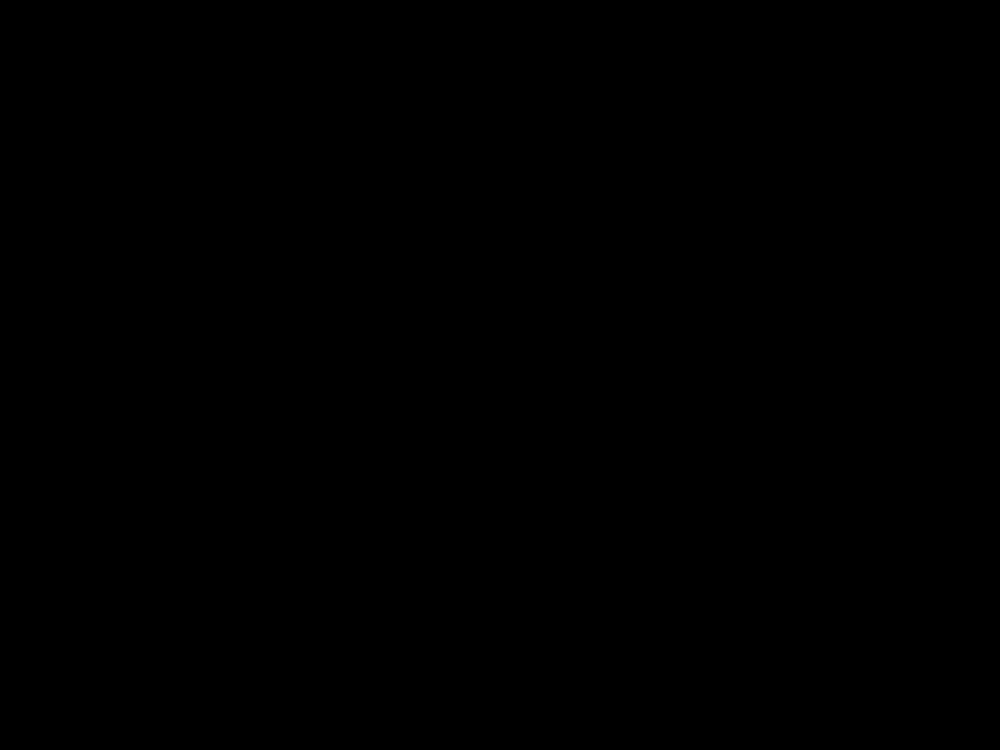
\includegraphics[width=30mm]{images/placeholder.png}}}%
%   \qquad
%   \subfloat[caption 2]{{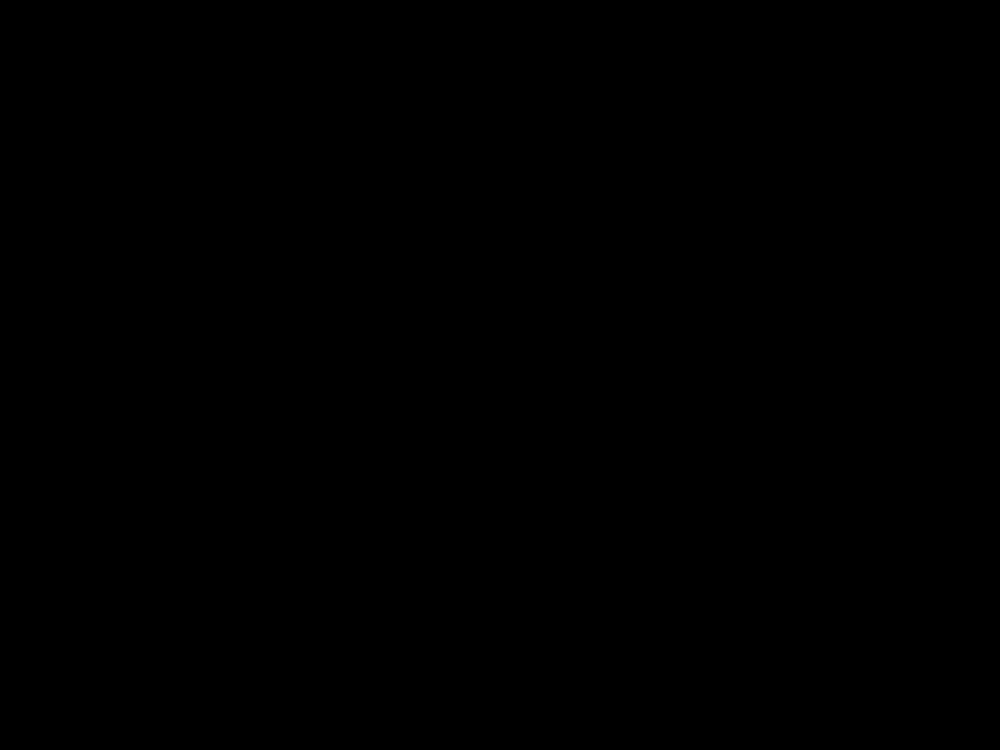
\includegraphics[width=30mm]{images/placeholder.png}}}%
%   \caption{Description}
% \end{figure}

% \begin{figure}[h]
%   \centerline{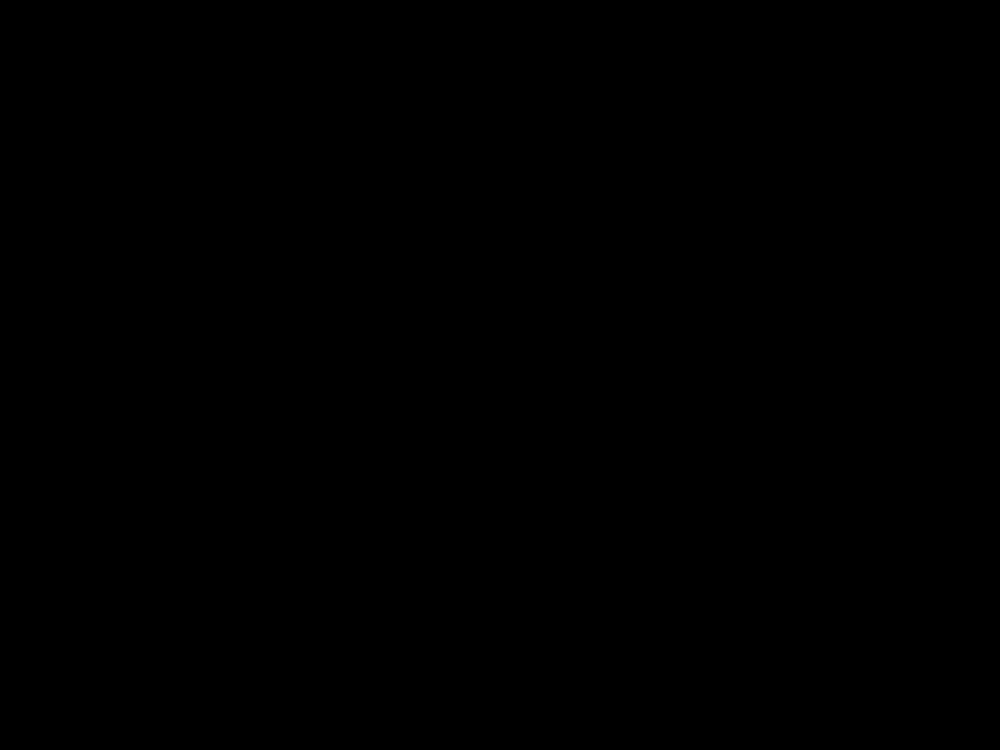
\includegraphics[width=50mm]{images/placeholder.png}}
%   \caption{Description}
% \end{figure}

%Template for a simple table 
%\begin{table}[h]
%   \caption{Description} %title of the table
%   \centering % centering table
%   \begin{tabular}{l rr} % creating three columns
%     \hline\hline %inserting double-line
%     & & \\ [0.5ex] % Insert half line vertical spacing
%     \hline % inserts single-line
%     & & \\ 
%     & & \\
%     & & \\
%     & & \\
%   \hline % inserts single-line
%   \end{tabular}
%   \label{tab:hresult}
% \end{table}
%-----------------------------------------------

\begin{document}
\setcounter{section}{1}

\section{Series}


\subsection{Defining a series}
A series is constructed by taking some sequence and summing all the terms of said sequence together. For example: let $\{ a_n \}$ be a sequence. Then:
\begin{align*}
  s_1 &= a_1\\
  s_2 &= a_1 + a_2\\
  s_3 &= a_1 + a_2 + a_3\\
  &\vdots\\
  s_n &= a_1 + a_2 + \cdots + a_n
\end{align*}
Which is then usually written more compactly as:
\begin{equation*}
  s_n = \sum_{i=1}^{n} a_i
\end{equation*}
Summing the first $n$ terms of a series is called a \textbf{partial sum}. We are usually interested in what happens when $n\to \infty$. We can extrapolate how a series behaves when $n$ goes to $\infty$ by studying the partial sum. If the partial sum is convergent/divergent, then when $n\to \infty$ the series will also be convergent/divergent. When a series is convergent we call the limit of the series $s$.
\begin{equation*}
  s = \sum_{n=1}^{\infty} a_n = \lim_{n\to\infty} s_n = \lim_{n\to\infty} \sum_{i=1}^{n} a_i
\end{equation*}


\subsection{Geometric Series}
An important example of an infinite sum is a geometric sequence. For a geometric series all the terms in the series share a common ratio $r$:
\begin{equation*}
  a + ar + ar^2 + ar^3 + \cdots = \sum_{k=0}^{\infty} ar^k
\end{equation*}
if $r\neq 1$ we get the following partial sum:
\begin{equation*}
  s_n = a + ar + ar^2 + ar^3 + \cdots + ar^n
\end{equation*}
Additionally we can multiply this series with $r$ to get:
\begin{equation*}
  rs_n = ar + ar^2 + ar^3 + \cdots + ar^{n+1}
\end{equation*}
We can now take the difference of these 2 series and we end up with:
\begin{align*}
  s_n - rs_n = (1 - r)s_n &= (a + \cancel{ar} + \cancel{ar^2} + \cancel{\cdots} + \cancel{ar^n}) - (\cancel{ar} + \cancel{ar^2} + + \cancel{ar^3} + \cancel{\cdots} + ar^{n+1})\\
  &= a(1 - r^{n+1})
\end{align*}
We can simplify this to find an expression for $s_n$:
\begin{equation*}
  s_n = \frac{a(1-r^{n+1})}{1-r}
\end{equation*}
From this we can see that the geometric series $\sum_{n=1}^\infty ar^{n-1}$ is convergent for $|r| < 1$ and will be equal to:
\begin{equation*}
  \sum_{n=1}^\infty ar^{n-1} = \frac{a}{1-r} \qquad \text{for} \; |r| < 1
\end{equation*}
if $|r|\geq 1$ the series is divergent and will go to either plus or minus $\infty$.
\begin{figure}[H]
  \centering
  \subfloat[$|r| < 1$]{{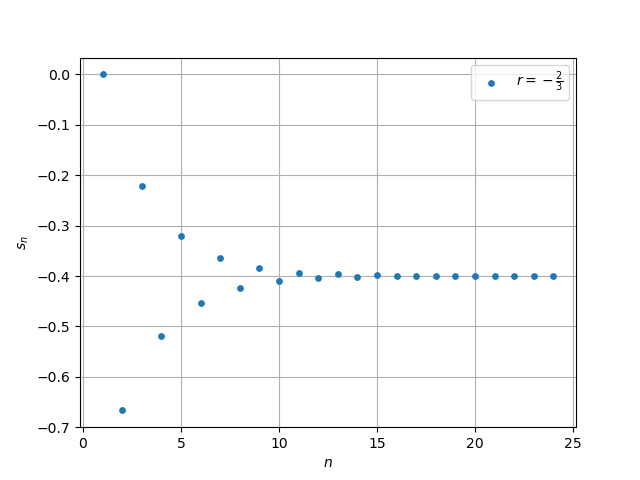
\includegraphics[width=80mm]{images/r_smaller_then_1.png}}}%
  \qquad
  \subfloat[$|r| \geq 1$]{{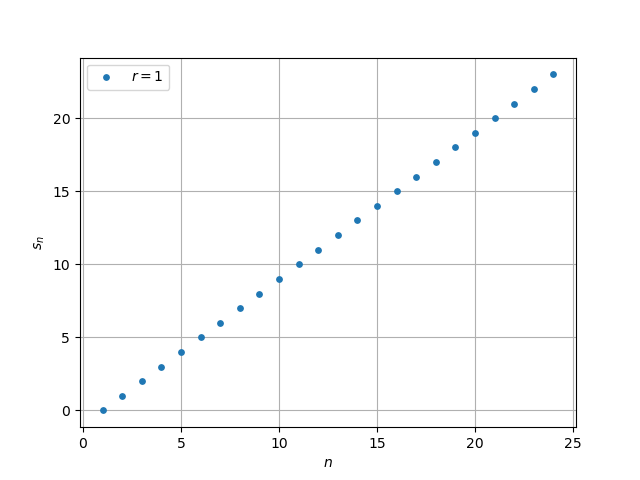
\includegraphics[width=80mm]{images/r_is_1.png}}}%
  \caption{Visualization of the geometric series for a value of $|r|$ smaller then one and for $|r|$ greater or equal to $1$. Note that the series where $r=1$ the value goes of to infinity.}
\end{figure}


\subsection{Telescoping series}
A telescoping series is a series of the form:
\begin{equation*}
  \sum_{n=1}^\infty \frac{1}{n(n+1)} = \frac{1}{2} + \frac{1}{6} + \frac{1}{12} + \cdots
\end{equation*}
The partial sum will be the first $k$ terms of the series:
\begin{equation*}
  s_n = \sum_{k=1}^{n} \frac{1}{k(k+1)}
\end{equation*}
We can use partial fraction decomposition to find that:
\begin{equation*}
  \frac{1}{k(k+1)} = \frac{1}{k} + \frac{1}{k+1}
\end{equation*}
The partial sum $s_n$ will then be:
\begin{align*}
  s_n &= \left(\frac{1}{1} - \cancel{\frac{1}{2}}\right) + \left(\cancel{\frac{1}{2}} - \cancel{\frac{1}{3}}\right) + \cancel{\cdots} + \left(\cancel{\frac{1}{n}} - \frac{1}{n+1}\right)\\
      &= 1 - \frac{1}{n+1}
\end{align*}
When we take the limit of this partial sum as $n$ goes to infinity we find:
\begin{equation*}
  \lim_{n\to\infty}s_n = \lim_{n\to\infty} 1 - \frac{1}{n+1} = 1
\end{equation*}
Thus this series converges to $1$.


\subsection{Harmonic series}
The harmonic series is given as:
\begin{equation*}
  \sum_{n=1}^{\infty} \frac{1}{n} = 1 + \frac{1}{2} + \frac{1}{3} + \cdots + \frac{1}{k} + \cdots
\end{equation*}
We recognize that the sum forms a rough estimation of the area of the curve given as $y = \frac{1}{x}$. Since it's an approximation we know that the series will always be larger then the area under te curve. Hence:
\begin{equation*}
  \sum_{n=1}^{\infty} \frac{1}{n} > \int_0^\infty \frac{1}{x} \d x
\end{equation*}
We can solve this integral easily as follows:
\begin{align*}
  \int_0^\infty \frac{1}{x} \d x &= \lim_{t\to\infty}\int_0^t \frac{1}{x} \d x\\
                                 &= \lim_{t\to\infty} \ln(t) = \infty
\end{align*}
Since $\sum_{n=1}^{\infty} 1/n > \int_0^\infty 1/x \d x$ we can assert for sure that the limit of the series must also be infinity.


\subsection{The general term test}
If $\{ a_n \}$ is some sequence and $s_n$ is a series constructed from said sequence that converges, then $\lim_{n\to\infty} a_n = 0$. This can also be formulated the other way around as: if $\lim_{n\to\infty} a_n$ does not exists or if $\lim_{n\to\infty} a_n \neq 0$ then the series $s_n$ is divergent.  This is because the sum will keep getting larger and larger if the sequence does not converge to $0$. Important side note: A geenral term of $0$ of some sequence $\{ a_n \}$ does not tell you anythin about whether the series converges or diverges.
\begin{figure}[h]
  \centerline{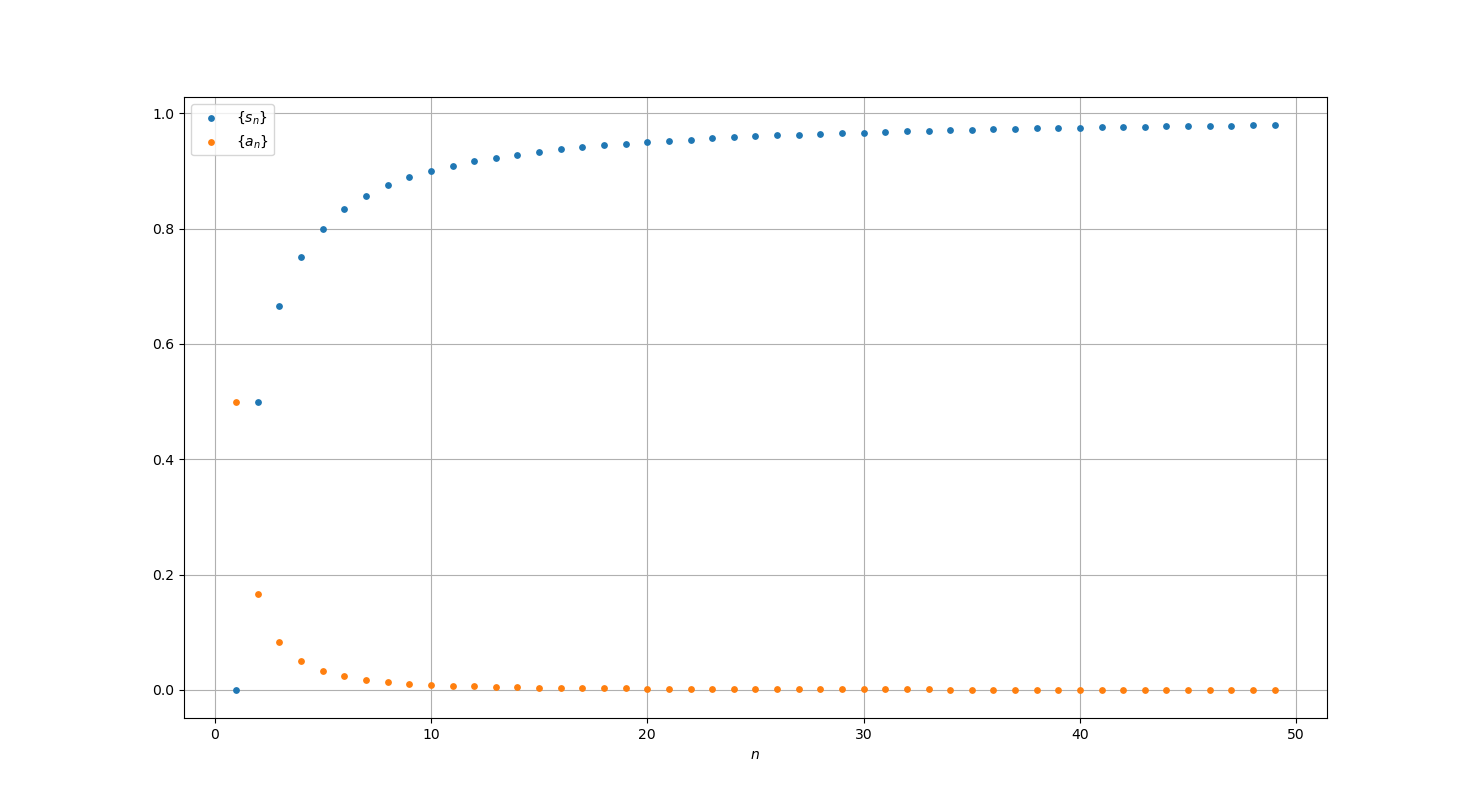
\includegraphics[width=150mm]{images/Converging_visualization.png}}
  \caption{The relation between the convergence of the sequence $\{ a_n \} = \frac{1}{n(n+1)}$ and the convergence of the series $\{ s_n \} = \sum_{i=1}^{n}\frac{1}{i(i+1)}$ visualized.}
\end{figure}


\subsection{Algebraic rules for manipulating series}
Let $\sum_{n=1}^{\infty} a_n = S \in \R$, $\sum_{n=1}^{\infty} b_n = T \in \R$ and $c_1,c_2 \in \R$, then the following rules apply:
\begin{itemize}
  \item $\sum_{n=1}^{\infty} c_1a_n = c_1\sum_{n=1}^{\infty} a_n = c_1S$
  \item $\sum_{n=1}^{\infty} (a_n \pm b_n) = \sum_{n=1}^{\infty} a_n \pm \sum_{n=1}^{\infty} b_n = S \pm T$
  \item $\sum_{n=1}^{\infty} (c_1a_n \pm c_2b_n) = c_1\sum_{n=1}^{\infty} a_n \pm c_2\sum_{n=1}^{\infty} b_n = c_1S \pm c_2T$
\end{itemize}
Note that these always apply when $a_n$ and $b_n$ both converge.
\end{document}